While pipelines designs continue to improve, memory technology has been struggling to keep up with the increase in clock speed and performance.
Even though memory bandwidth can be improved with more bank parallelization, the memory latency remains the bottle neck to really improving memory performance.
Common memory technologies used in embedded systems contain a significant trade off between access latency and capacity. 
Static Random-Access Memories (SRAM) provides sufficient latency that allows single cycle memory access latencies from the pipeline.
However, the hardware cost to implement each memory cell prohibits large capacities to be implemented close to the processor.
On the other hand, Dynamic Random-Access Memories (DRAM) uses a compact memory cell design that can easily be designed into larger capacity memory blocks.
But the memory cell of DRAMs must be constantly refreshed due to charge leakage, and the large capacity of DRAM cells in a memory block design often prohibit faster access latencies.
%TODO: talk about about embedded systems seldom need disk?
To bridge the latency gap between the pipeline and memory, smaller memories are placed in between the pipeline and larger memories to act as a buffer, forming a memory hierarchy.
The smaller memories give faster access latencies at the cost of lower capacity, while larger memories make up for that with larger capacity but slower access latencies. 
The goal is to speed up program performance by placing commonly accessed values closer to the pipeline, while less access values are placed farther away.

\subsection{Caches vs. Scratchpads}
\begin{wrapfigure}{r}{0.5\textwidth}
  \vspace{-20pt}
  \begin{center}
    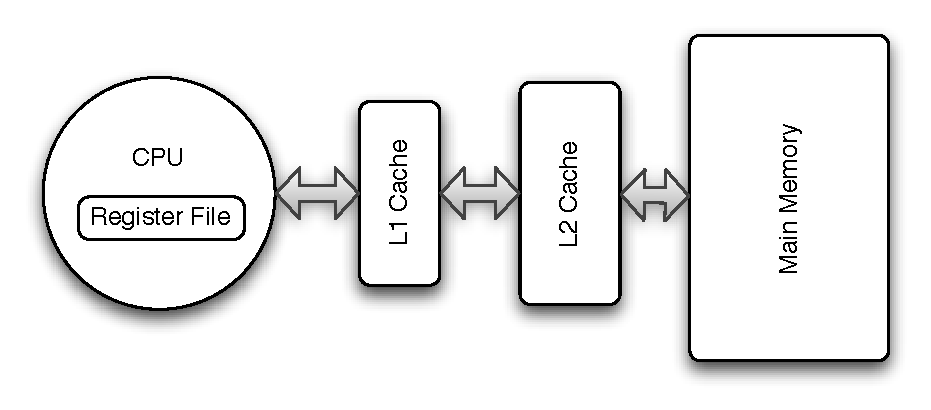
\includegraphics[scale=.5]{figs/conventional_mem_hierarchy}
  \end{center}
  \vspace{-20pt}
  \caption{Memory Hierarchy w/ Caches}
  \label{fig:conventional_mem_hierarchy}
  \vspace{-10pt}
\end{wrapfigure}   
A \emph{CPU Cache} (or cache) is commonly used in the memory hierarchy to manage the smaller fast access memory made of SRAMs.
The cache manages of contents of the fast access memory in hardware by leveraging the spatial and temporal locality of data accesses. 
The main benefits of the cache is that it abstracts away the memory hierarchy from the programmer.
When a cache is used, all memory accesses is routed through the cache. 
If the data from the memory access is on the cache, then a cache hit occurs, and the data is returned right away.
However, if data is not on the cache, then a cache miss occurs, and the cache controller fetches the data from the larger memory and adjusts the memory contents on the cache. 
The replacement policy of the cache is used to determine which cache line, the unit of memory replacement on caches, to replace. 
A variety of cache replacement policies have been researched~\todo{cite} and used to optimize for memory access patterns of different applications. 
In fact, modern memory hierarchies often contain multiple layers of hierarchy to balance the trade-off between speed and capacity.
A commonly used memory hierarchy is shown in figure~\ref{fig:conventional_mem_hierarchy}.
If the data value is not found in the L1 cache, then it is searched for in the L2 cache. 
If the L2 cache also misses, then the data is retrieved from main memory, and sent back to the CPU while the L1 and L2 cache updates its contents.
Often times different replacement policies are used at different levels of the memory hierarchy to optimize the hit rate or miss latency of the memory access. 
As sophisticated as this seems, the programmer is oblivious to the different levels of memory hierarchy, and whether or not an access hits the cache or goes all the way out to main memory. 
The memory hierarchy is hidden from the programmer, and the hardware gives its best-effort to optimize memory access latencies without any guarantees.
%talk about cache timing analysis and why it is difficult
%caches also cause other issues - multi threading shared cache, multi core cache coherint

%Introduce scratchpads. uses same technology, but is used for power saving from the circuitry
% Expose the memory hierarchy to the programmer, at the expense of more work from the programmer, but have better control over time 

%discuss possible ways to manage scratchpads, programming models, embedded systems often require in depth anaysis of memory access paterns already etc

%Summarize that the unpredictablility from caches does not stem from the memory technology, but how it is managed by the hardware. 
% That's why using scratchpads exposes the memory hierarchy to the programmer, while still allowing the benefits of smaller, faster memories
% The unpredictability of DRAM technology however stems from the actual memory technology, so we explain the basics of DRAM a little more 
\subsection{DRAM Memory Controller}
% first discuss the basics of DRAM technology, explaining what makes accesses unpredictable

% talk about the back end controller to implement predictable access latencies

% mentions that we will discuss the details and the integration with the PTARM arhictecture in the next section
